\documentclass[a4,10pt]{article}

\usepackage{graphicx}
\usepackage{epstopdf}
\usepackage{times}
\usepackage{rotating}


\begin{document}

\begin{sidewaystable}[p]
\tiny{\begin{tabular}{|c|c|c|c|c|c|c|c|c|c|c|c|c|c|c|c|c|c|c|c|}
 & >p/k & <p/k & >k/100 & <k/100 & k/100 & sum & cnt & avg & prod & <k & p/k & most & >k & few & -est & k & the & some & all\\
\hline
brown. & 38 & 22 & 2 & 18 & 8 & 28 & 354 & 34 & 19 & 490 & 688 & 1532 & 1122 & 3451 & 4368 & 16455 & 63376 & 81693 & 202587\\
wacky. & 16134 & 15120 & 708 & 738 & 157 & 859 & 25050 & 641 & 738 & 81014 & 75046 & 100530 & 161578 & 136270 & 178004 & 357629 & 278640 & 1218302 & 2910784\\
\hline
total & 16172 & 15142 & 710 & 756 & 165 & 887 & 25404 & 675 & 757 & 81504 & 75734 & 102062 & 162700 & 139721 & 182372 & 374084 & 342016 & 1299995 & 3113371
\end{tabular}}
\end{sidewaystable}



\vspace{0.2cm}

\begin{center}
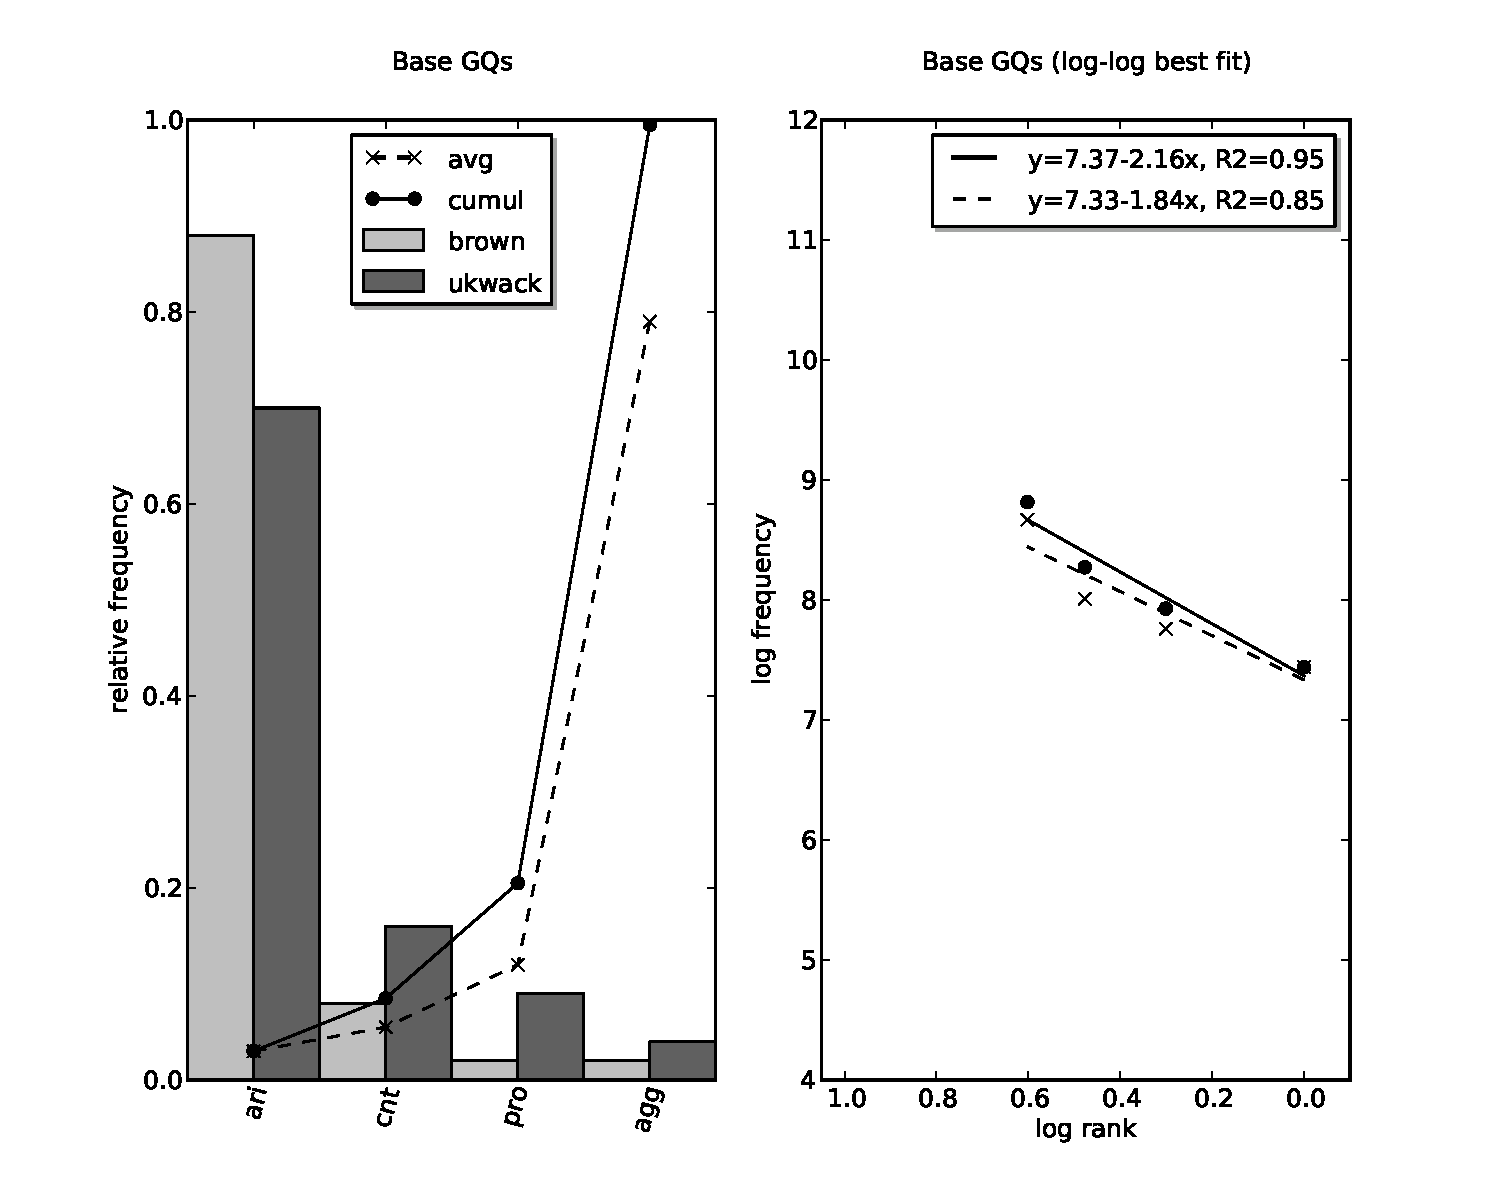
\includegraphics[scale=0.5]{/home/professors/cathorne/Desktop/quantifiers/wacky-script/plotting-extra/Base-GQs-stats.pdf}
\end{center}

\end{document}